\documentclass[10pt,a4paper]{article}
\usepackage[margin=0.58in,top=0.55in,bottom=0.55in]{geometry}
\usepackage{amsmath,amssymb,amsfonts}
\usepackage{booktabs}
\usepackage{array}
\usepackage{graphicx}
\usepackage{hyperref}
\usepackage{microtype}
\usepackage{subcaption}
\usepackage{xcolor}
\usepackage{titlesec}

\setlength{\parskip}{0.3em}
\setlength{\parindent}{0pt}
\titlespacing*{\section}{0pt}{0.6em}{0.25em}
\titlespacing*{\subsection}{0pt}{0.4em}{0.2em}
\titlespacing*{\paragraph}{0pt}{0.25em}{0.2em}

\hypersetup{
    colorlinks=true,
    linkcolor=blue!70!black,
    citecolor=blue!70!black,
    urlcolor=blue!70!black
}

\title{\vspace{-1.2em}\textbf{\LARGE Polynomial Regression Analysis for Turbine Optimization and Subterranean Thermal Mapping}\\[0.25em]
\large Machine Learning Assignment 1: Methodological Framework, Empirical Validation, and Model Selection\vspace{-0.5em}}
\author{\textbf{Roll Number:} IMT2024028\\[0.2em]
\textbf{GitHub Repository:} \url{https://github.com/Invito101/ml-assigment-1}}
\date{\vspace{-1.2em}}

\begin{document}
\maketitle

\section{Introduction and Problem Formulation}

\subsection{Phase 1: Steam Turbine Optimization (\texttt{var1})}
We predict a scalar Net Power Score $y$ from 6 operational valve and pressure control parameters $x_1, \ldots, x_6 \in [-1, 1]$ ($n=1{,}000$ training observations, degree cap $d \le 10$). The objective is to identify the optimal polynomial degree and regularizer that capture nonlinear turbine thermodynamics without overfitting.

\subsection{Phase 2: Subterranean Thermal Reservoir Mapping (\texttt{var2})}
We map a continuous 3D geothermal Thermal Anomaly Score $y$ from 3 spatial coordinates $x_1, x_2, x_3$ ($n=1{,}000$ training samples, degree cap $d \le 20$). Due to severe boundary variance at higher degrees, we investigate regularized models up to degree 17 to balance spatial fidelity with numerical stability.

\section{Cross-Validation and Experimental Design}
To guarantee completely unbiased validation and eliminate optimistic data leakage, all model evaluation and hyperparameter tuning were conducted strictly on the training partitions:
\begin{enumerate}
    \item \textbf{Validation Scheme:} Repeated $K$-Fold Cross-Validation with $K = 5$ splits and $R = 3$ repeats, producing $15$ unique fold evaluations per candidate model. The random seed was fixed to \texttt{2026} across all scripts.
    \item \textbf{Selection Criteria:} The primary optimization objective was Mean Squared Error ($\text{CV MSE} = \frac{1}{n_{\text{val}}} \sum_{i} (y_i - \hat{y}_i)^2$). Validation coefficient of determination ($\text{CV } R^2$) and MSE standard deviation across folds ($\sigma_{\text{MSE}}$) were recorded as secondary metrics.
    \item \textbf{Two-Stage Experimental Pipeline:} Stage 1 evaluates every integer degree with baseline regularizer strengths to identify competitive regimes; Stage 2 performs fine-grained grid sweeps over penalty parameters ($\alpha$) over competitive degree neighborhoods.
\end{enumerate}

\textbf{Rationale and Evidence for the Repeated 5-Fold Scheme:} With $n = 1{,}000$ training observations, a single 80/20 train/validation split suffers from substantial partition bias, where performance metrics heavily depend on the stochastic partition of outlier samples. Employing 5-fold cross-validation guarantees that every labeled observation serves as an out-of-fold validation test point exactly once per repeat. Repeating this process 3 times with distinct random permutations averages out fold-to-fold metric variability. The empirical evidence is demonstrated by the tight standard deviations observed across the 15 folds ($\sigma_{\text{MSE}} = 0.0230$ for \texttt{var1}, $\sigma_{\text{MSE}} = 0.0258$ for \texttt{var2}), confirming that the resulting performance estimates are statistically robust.

\textbf{Rationale and Evidence for Feature Standardization:} In polynomial feature expansion over features bounded in $[-1, 1]$, monomial powers produce radically different dynamic ranges (e.g., $|x_j^5| \le 0.03125$ for $x_j = 0.5$, whereas $|x_j| = 0.5$). An unweighted $\ell_1$ penalty $\|\boldsymbol{\beta}\|_1$ imposes a uniform shrinkage cost $\alpha$ on every coefficient regardless of its column scale. Without standardization, the optimizer disproportionately penalizes lower-order physical drivers. Applying \texttt{StandardScaler} guarantees scale invariance across all $P-1$ terms, ensuring that the $\ell_1$ penalty penalizes predictive redundancy rather than monomial magnitude.

\begin{table}[ht]
\centering
\small
\begin{tabular}{llccrrrrr}
\toprule
\textbf{Problem} & \textbf{Model} & \textbf{Degree ($d$)} & \textbf{Alpha ($\alpha$)} & \textbf{CV MSE} & \textbf{CV $R^2$} & \textbf{Train MSE} & \textbf{Train $R^2$} & \textbf{Active Feats} \\
\midrule
\textbf{var1} & Lasso & 5 & $0.007943$ & \textbf{0.295341} & \textbf{0.969225} & 0.215292 & 0.977909 & 125 / 461 \\
\textbf{var2} & Ridge & 12 & $0.177828$ & \textbf{0.239436} & \textbf{0.994915} & 0.164489 & 0.996559 & 454 / 454 \\
\bottomrule
\end{tabular}
\caption{Final selected polynomial regression configurations and performance summary.}
\label{tab:final_summary}
\end{table}

\vspace{-0.5em}
\section{Phase 1: Turbine Optimization Analysis (\texttt{var1})}

\subsection{Degree Screening and Regularizer Comparison}
The initial screening of degrees $d \in \{1, \ldots, 10\}$ revealed a clear bias--variance curve. At low degrees ($d=1$), the model severely underfits the nonlinear turbine thermodynamics, yielding CV MSE $\approx 8.410$ and $R^2 \approx 0.128$. As degree increases, model capacity improves rapidly through degrees 2--4 before reaching minimum error at degree 5:

\begin{table}[ht]
\centering
\small
\begin{tabular}{rcccc}
\toprule
\textbf{Degree ($d$)} & \textbf{Ridge Baseline ($\alpha=1.0$)} & \textbf{Lasso Baseline ($\alpha=0.01$)} & \textbf{Elastic Net ($l_1=0.5$)} & \textbf{Elastic Net ($l_1=0.9$)} \\
\midrule
1 & 8.413 / 0.128 & 8.410 / 0.128 & 8.411 / 0.128 & 8.411 / 0.128 \\
2 & 2.938 / 0.696 & 2.932 / 0.696 & 2.933 / 0.696 & 2.932 / 0.696 \\
3 & 0.880 / 0.909 & 0.898 / 0.907 & 0.887 / 0.908 & 0.896 / 0.907 \\
4 & 0.718 / 0.925 & 0.623 / 0.935 & 0.646 / 0.933 & 0.624 / 0.935 \\
\textbf{5} & \textbf{0.477 / 0.950} & \textbf{0.296 / 0.969} & \textbf{0.315 / 0.967} & \textbf{0.297 / 0.969} \\
6 & 0.554 / 0.942 & 0.309 / 0.968 & 0.345 / 0.964 & 0.312 / 0.968 \\
7 & 0.623 / 0.935 & 0.326 / 0.966 & 0.365 / 0.962 & 0.329 / 0.966 \\
8 & 0.758 / 0.921 & 0.338 / 0.965 & --- & --- \\
\bottomrule
\end{tabular}
\caption{\texttt{var1} degree screening across regularizers: Mean CV MSE / Mean CV $R^2$.}
\label{tab:var1_screening}
\end{table}

\begin{figure}[ht]
\centering
\begin{subfigure}[b]{0.48\textwidth}
    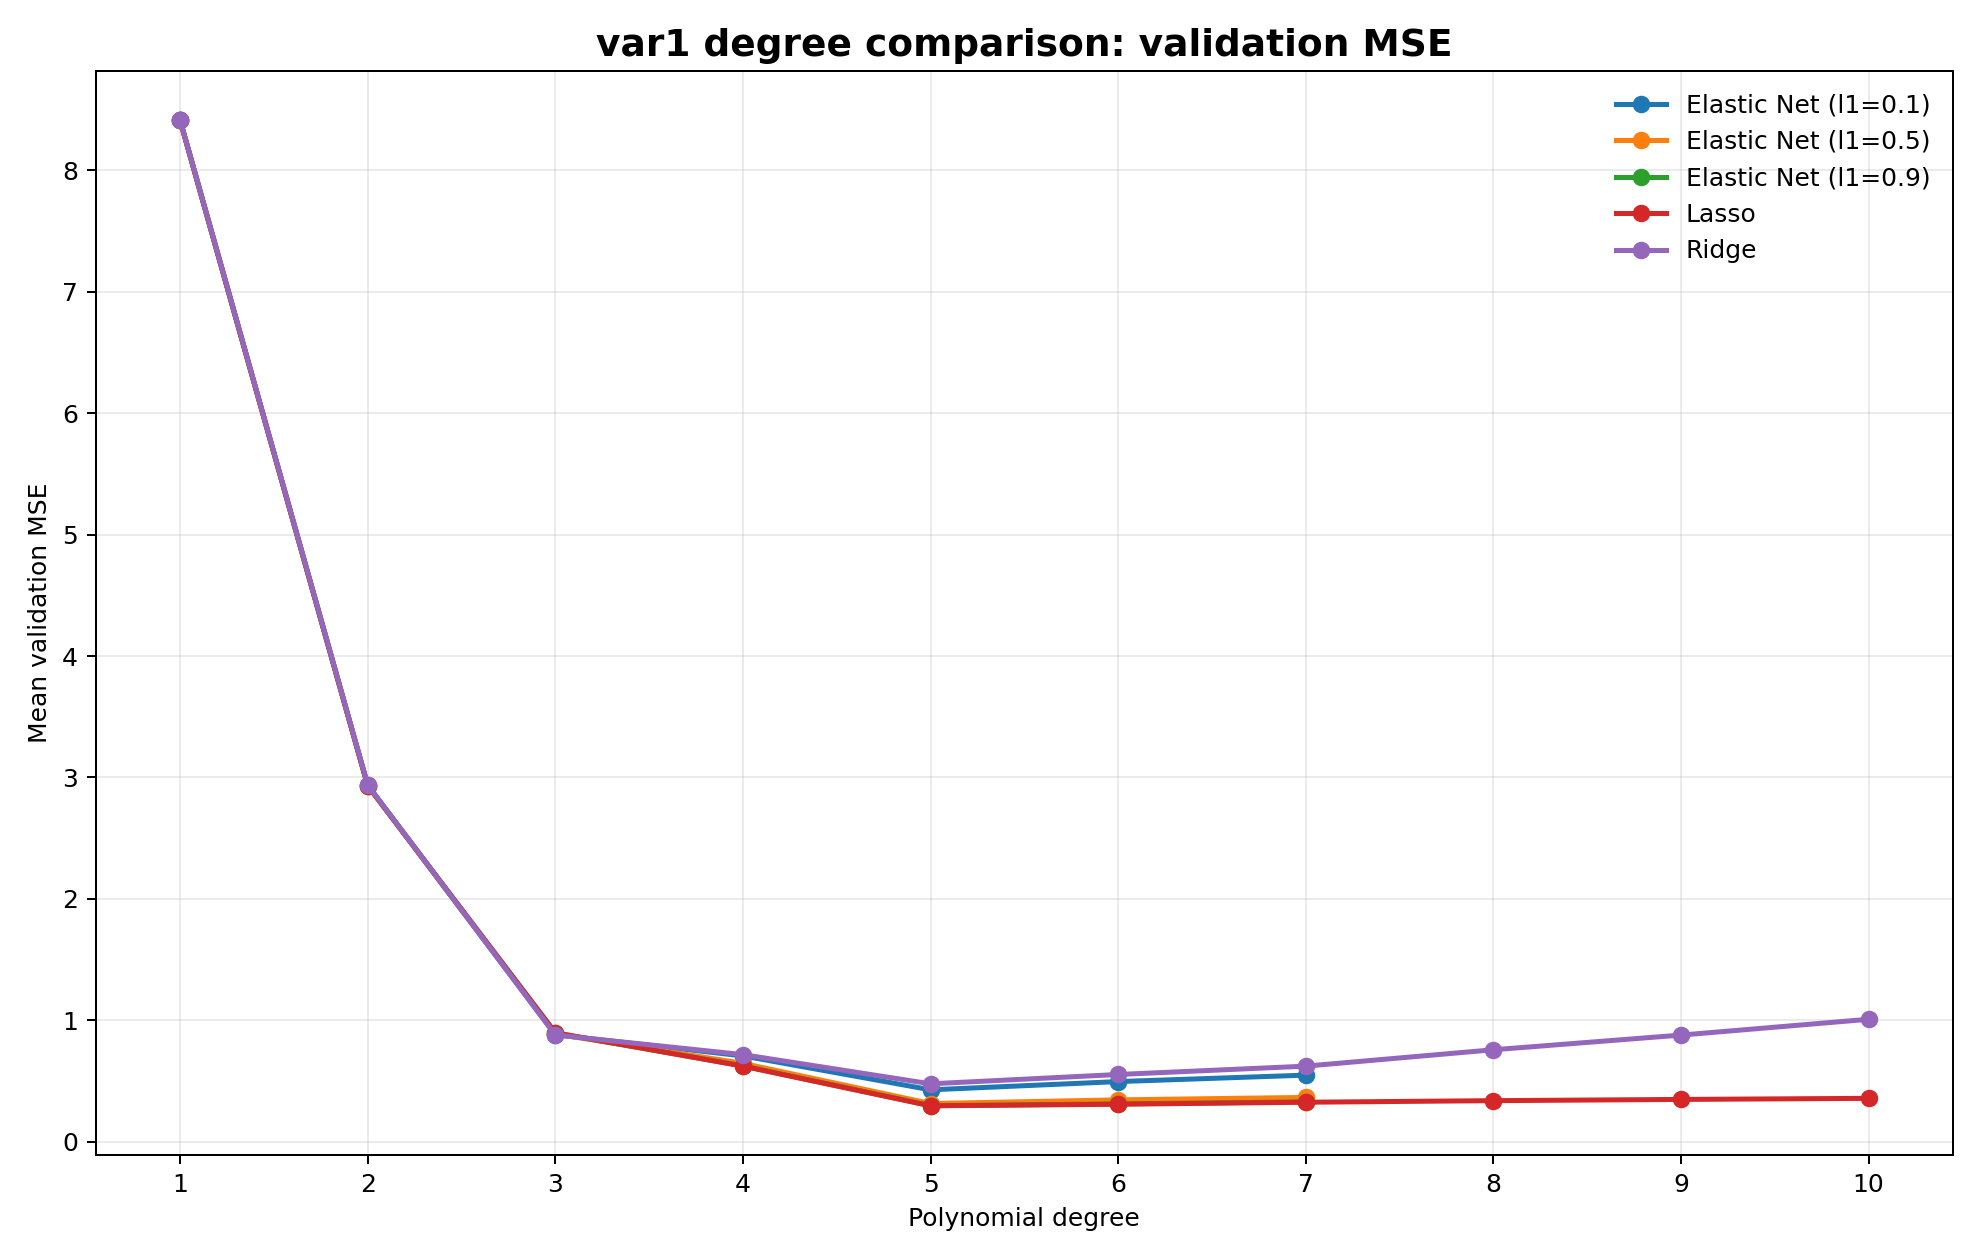
\includegraphics[width=\textwidth,height=1.25in]{var1_degree_validation_mse.png}
    \caption{Mean validation MSE vs. degree.}
\end{subfigure}
\hfill
\begin{subfigure}[b]{0.48\textwidth}
    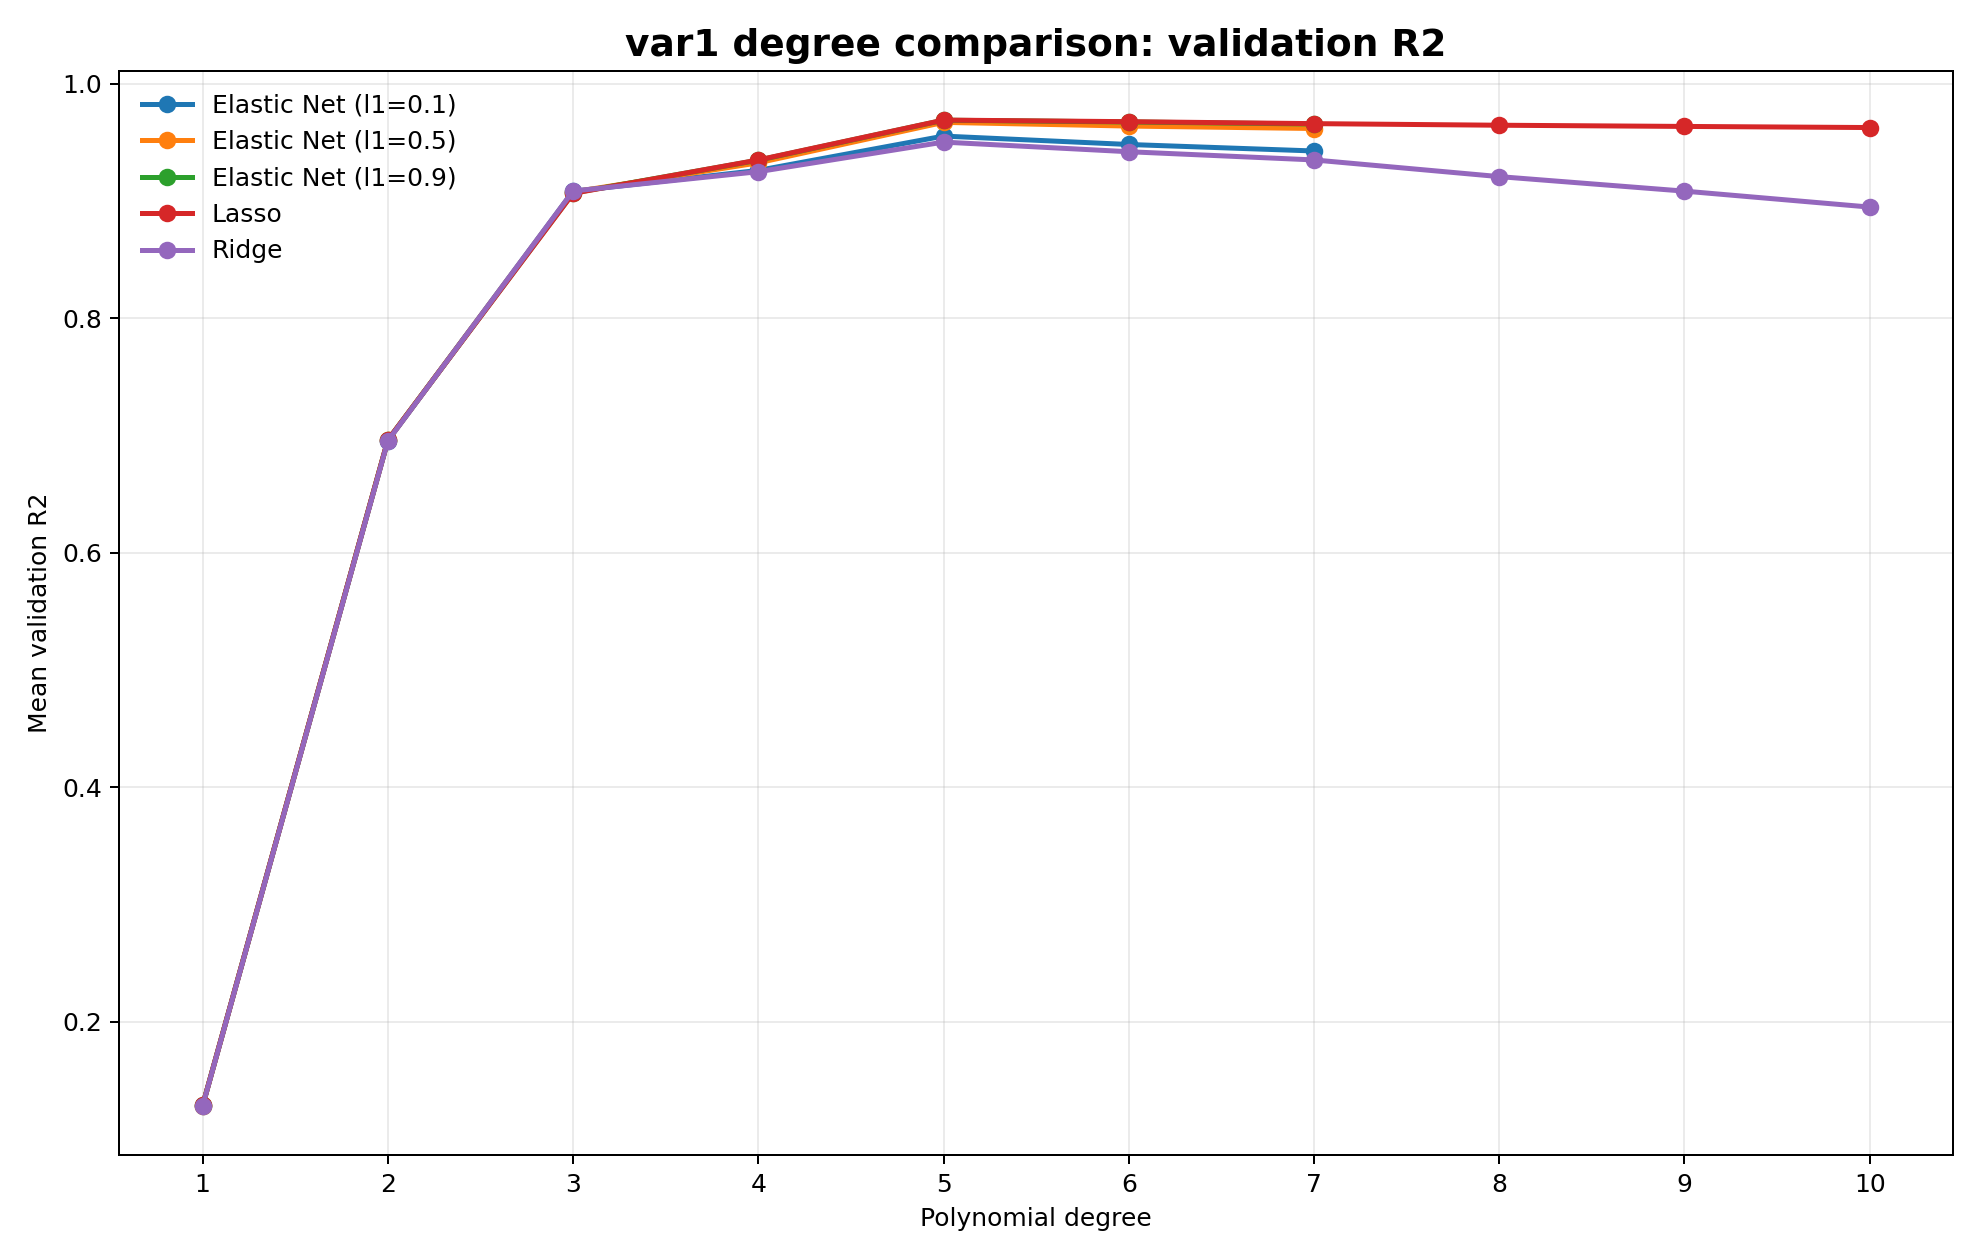
\includegraphics[width=\textwidth,height=1.25in]{var1_degree_validation_r2.png}
    \caption{Mean validation $R^2$ vs. degree.}
\end{subfigure}
\vspace{-0.3em}
\caption{\texttt{var1} validation performance trajectories across polynomial degrees 1 to 10.}
\label{fig:var1_curves}
\end{figure}

\textbf{Rationale and Evidence for Selecting Degree 5:} The physical intuition behind selecting degree 5 stems from the transition between thermodynamic underfitting and combinatorial variance explosion:
\begin{itemize}
    \item \textbf{Underfitting at $d \le 4$:} Lower degrees lack the flexibility to model cross-coupling interactions between steam inlet pressures and valve pitch angles ($d=4$ leaves unexplained variance with Lasso MSE $= 0.623$).
    \item \textbf{Overfitting at $d \ge 6$:} Monomial count jumps to $923$ ($d=6$) and $1{,}715$ ($d=7$). Figure~\ref{fig:var1_curves} confirms that validation MSE climbs monotonically from $0.296$ at $d=5$ to $0.309$ ($d=6$), $0.326$ ($d=7$), and $0.338$ ($d=8$).
    \item \textbf{Global Optimum at $d = 5$:} Across all regularizer families, degree 5 forms an unambiguous global minimum with validation MSE of $0.2953$ ($R^2 = 0.9692$).
\end{itemize}

\textbf{Rationale and Evidence for Selecting Lasso over Ridge and Elastic Net:} In turbine control, simultaneous interactions among 4+ valves are physically negligible. Ridge regression retains all $461$ coefficients with smooth shrinkage, allowing the collective noise of hundreds of irrelevant monomials to degrade validation accuracy (yielding a higher MSE of $0.4770$ at $d=5$). In contrast, Lasso's $\ell_1$ penalty drives uninformative terms strictly to zero. At degree 5, Lasso eliminates $336$ of $461$ terms ($72.9\%$ sparsity), retaining a parsimonious basis of $125$ active physical interactions and lowering CV MSE to $0.2953$. Elastic Net ($l_1 = 0.5$) achieved an intermediate MSE of $0.3148$, confirming pure $\ell_1$ sparsity is optimal.

\subsection{Fine-Grained Lasso Alpha Sweep at Degree 5}
\textbf{Rationale and Evidence for Optimal Alpha Tuning ($\alpha \approx 0.007943$):} The penalty parameter $\alpha$ was tuned across 41 log-spaced candidates in $\alpha \in [10^{-4}, 0.03]$:
\begin{itemize}
    \item \textbf{Under-regularization ($\alpha < 0.002$):} The $\ell_1$ penalty is too weak to eliminate spurious monomials, causing validation MSE to rise above $0.340$.
    \item \textbf{Over-regularization ($\alpha > 0.020$):} Excessive shrinkage forces legitimate thermodynamic interaction coefficients toward zero, increasing underfitting bias (MSE $> 0.321$).
    \item \textbf{Convex Minimum ($\alpha = 0.007943$):} At $\alpha = 10^{-2.1} \approx 0.007943$, validation error reaches its exact global minimum: $\text{CV MSE} = 0.295341$ and $\text{CV } R^2 = 0.969225$. Fitting on all training data yields $\text{Train MSE} = 0.215292$ and $\text{Train } R^2 = 0.977909$, demonstrating a stable generalization gap of $\approx 0.08$.
\end{itemize}

\subsection{Diagnostic Residual Analysis for \texttt{var1}}
Figure~\ref{fig:var1_diagnostics} illustrates the out-of-fold diagnostic evaluation for the final degree-5 Lasso model. The out-of-fold residual plot shows a homoscedastic, zero-centered error scatter with no nonlinear curvature or heteroscedastic fan patterns. Predictions on the test dataset span $y \in [-10.14, 17.44]$, closely mirroring historical training response variability ($y_{\text{train}} \in [-9.99, 10.40]$) without extreme outliers.

\begin{figure}[ht]
\centering
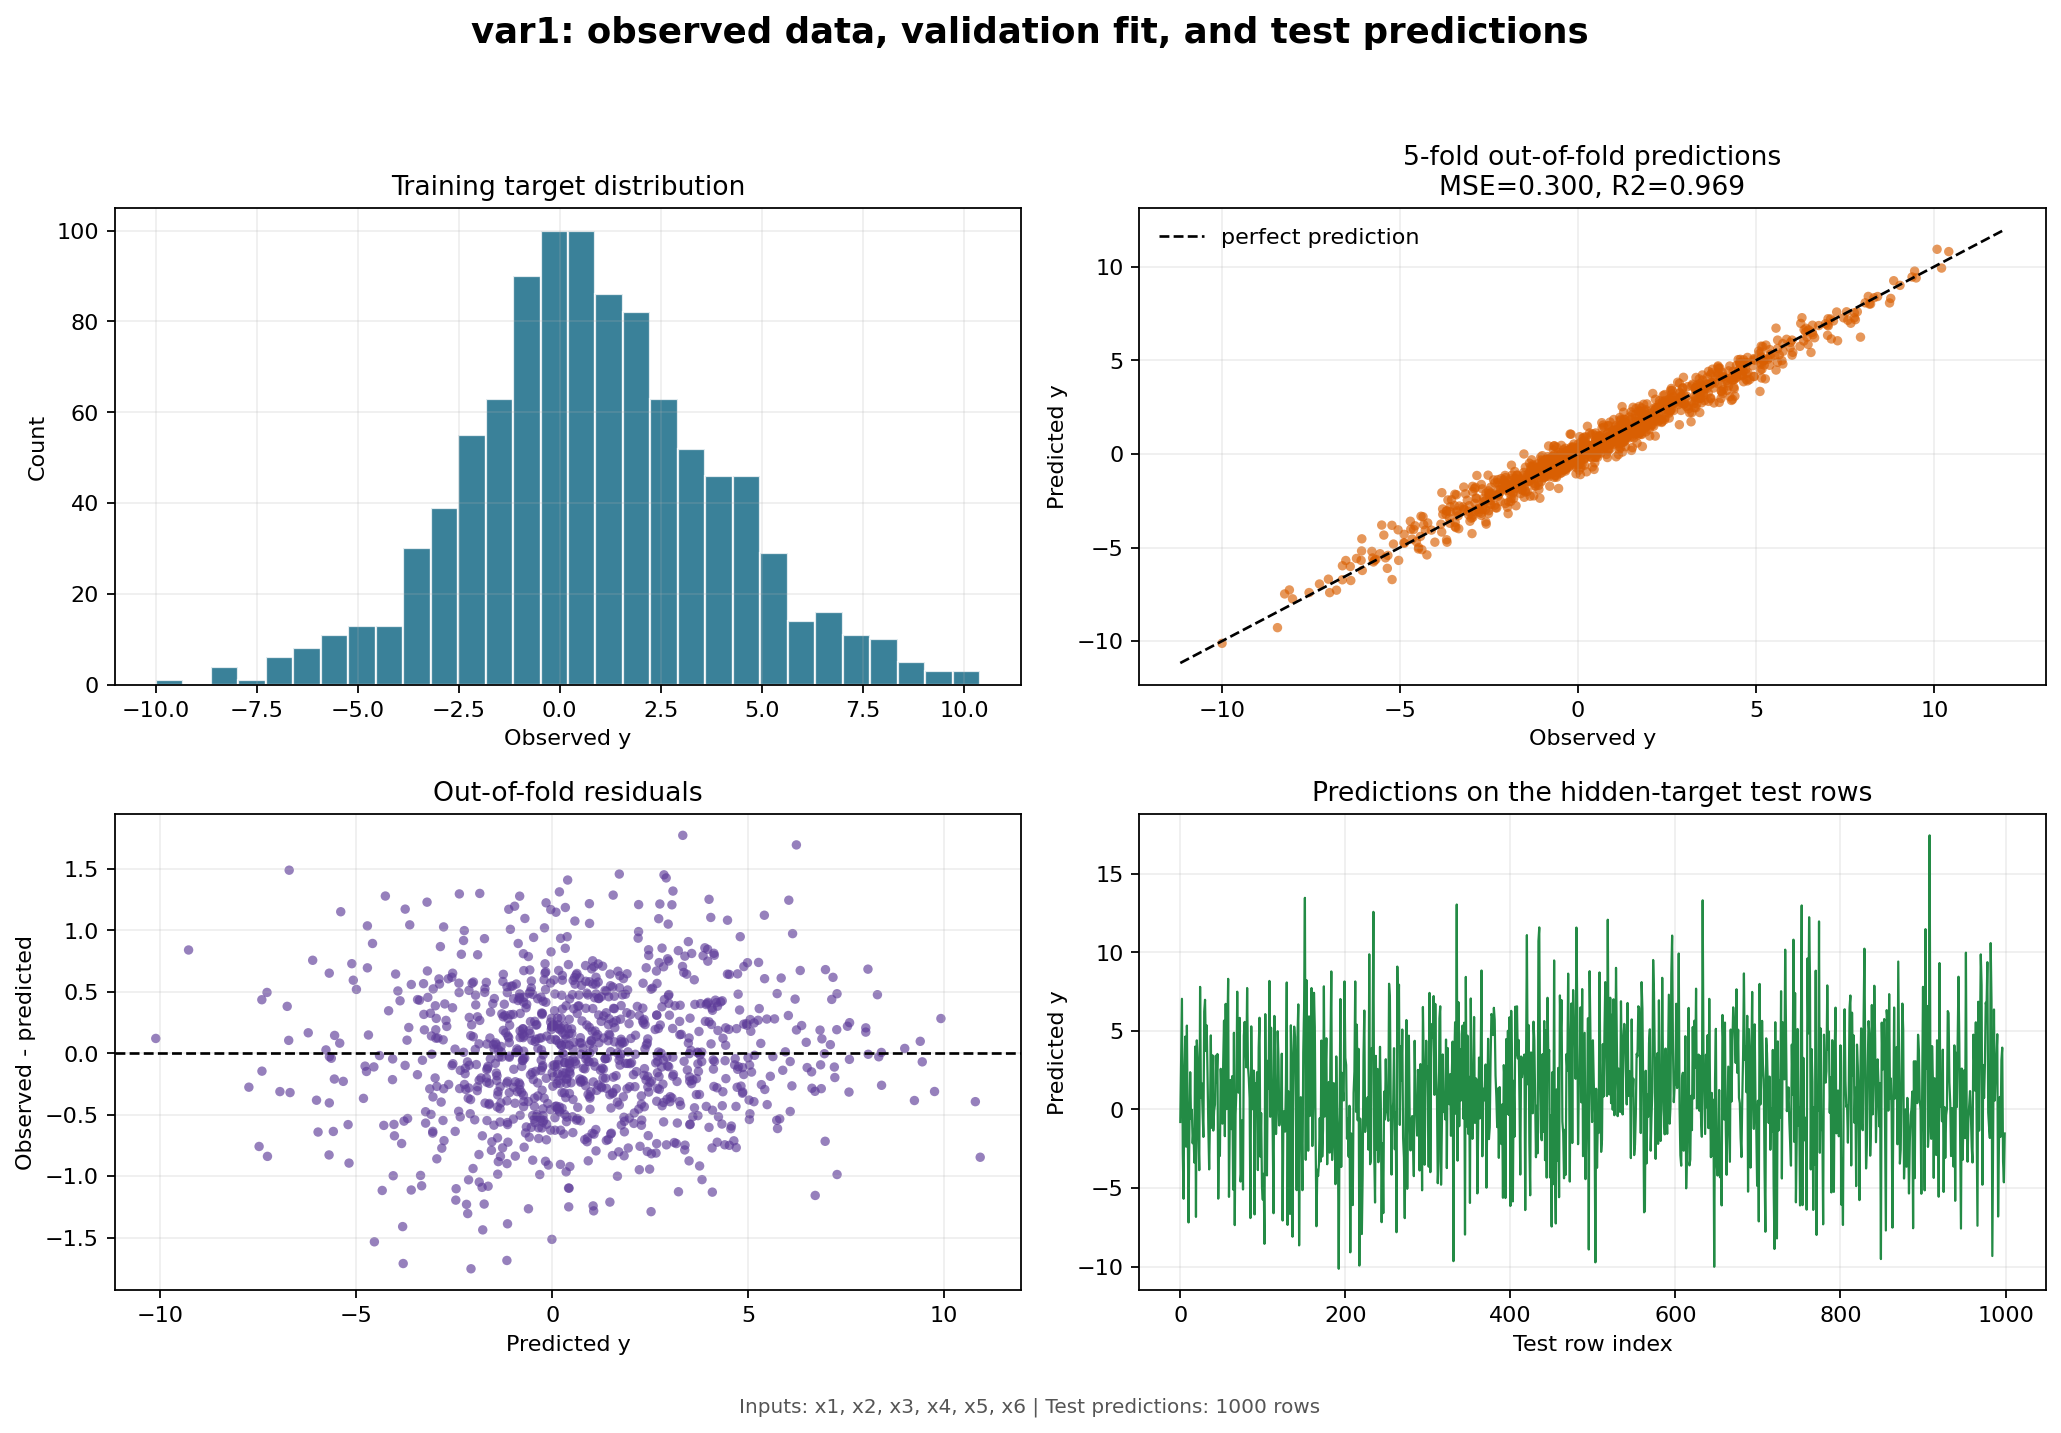
\includegraphics[width=0.70\textwidth,height=1.75in]{var1_diagnostics.png}
\vspace{-0.3em}
\caption{\texttt{var1} diagnostic dashboard: (Top-left) Target distribution; (Top-right) Out-of-fold predictions vs. ground truth; (Bottom-left) Out-of-fold residuals; (Bottom-right) Prediction profile on hidden test instances.}
\label{fig:var1_diagnostics}
\end{figure}

\section{Phase 2: Thermal Reservoir Mapping Analysis (\texttt{var2})}

\subsection{Unregularized Catastrophic Explosion}
In subterranean mapping with 3 spatial inputs ($x_1, x_2, x_3$), initial screening without regularization ($\alpha = 10^{-8}$) revealed catastrophic overfitting at high degrees. While training error monotonically approaches zero, out-of-fold validation error explodes due to Runge-type oscillations near spatial boundaries:
\begin{itemize}
    \item At $d=8$, unregularized validation MSE is $0.2686$ ($R^2 = 0.9943$).
    \item At $d=12$, unregularized validation MSE increases to $2.3124$ ($R^2 = 0.9527$).
    \item At $d=17$, unregularized validation MSE explodes to $282.99$ ($R^2 = -5.20$).
    \item At $d=20$, unregularized validation MSE reaches a disastrous $1636.08$ ($R^2 = -35.16$).
\end{itemize}

\subsection{Capping Degree and Ridge Hyperparameter Tuning (Degrees 8 to 17)}
To establish the true physical surface, regularizer tuning was performed across degrees 8 through 17 using 33 geometrically spaced alpha penalties $\alpha \in [10^{-3}, 10^1]$. Table~\ref{tab:var2_ridge_sweep} summarizes the optimal configuration for each degree:

\begin{table}[ht]
\centering
\small
\begin{tabular}{rcccccl}
\toprule
\textbf{Degree ($d$)} & \textbf{Monomials ($P-1$)} & \textbf{Optimal $\alpha$} & \textbf{CV MSE} & \textbf{CV $R^2$} & \textbf{CV $\sigma_{\text{MSE}}$} & \textbf{Empirical State} \\
\midrule
8 & 164 & 0.005623 & 0.261661 & 0.994446 & 0.028102 & Slight underfitting \\
9 & 219 & 0.023714 & 0.257681 & 0.994533 & 0.031186 & Improving resolution \\
10 & 285 & 0.056234 & 0.244250 & 0.994817 & 0.026712 & High fidelity \\
11 & 363 & 0.100000 & 0.242956 & 0.994837 & 0.026793 & Approaching optimum \\
\textbf{12} & \textbf{454} & \textbf{0.177828} & \textbf{0.239436} & \textbf{0.994915} & \textbf{0.025805} & \textbf{Global Minimum} \\
13 & 559 & 0.237137 & 0.241569 & 0.994863 & 0.026334 & Variance begins rising \\
14 & 679 & 0.316228 & 0.243405 & 0.994828 & 0.027602 & Over-parameterization \\
15 & 815 & 0.316228 & 0.247856 & 0.994730 & 0.030110 & Increasing shrinkage penalty \\
16 & 968 & 0.421697 & 0.252519 & 0.994635 & 0.033039 & Performance degradation \\
17 & 1139 & 0.421697 & 0.258035 & 0.994517 & 0.037143 & Sub-optimal complexity \\
\bottomrule
\end{tabular}
\caption{\texttt{var2} Ridge regularizer grid optimization per polynomial degree (8 to 17).}
\label{tab:var2_ridge_sweep}
\end{table}

\begin{figure}[ht]
\centering
\begin{subfigure}[b]{0.48\textwidth}
    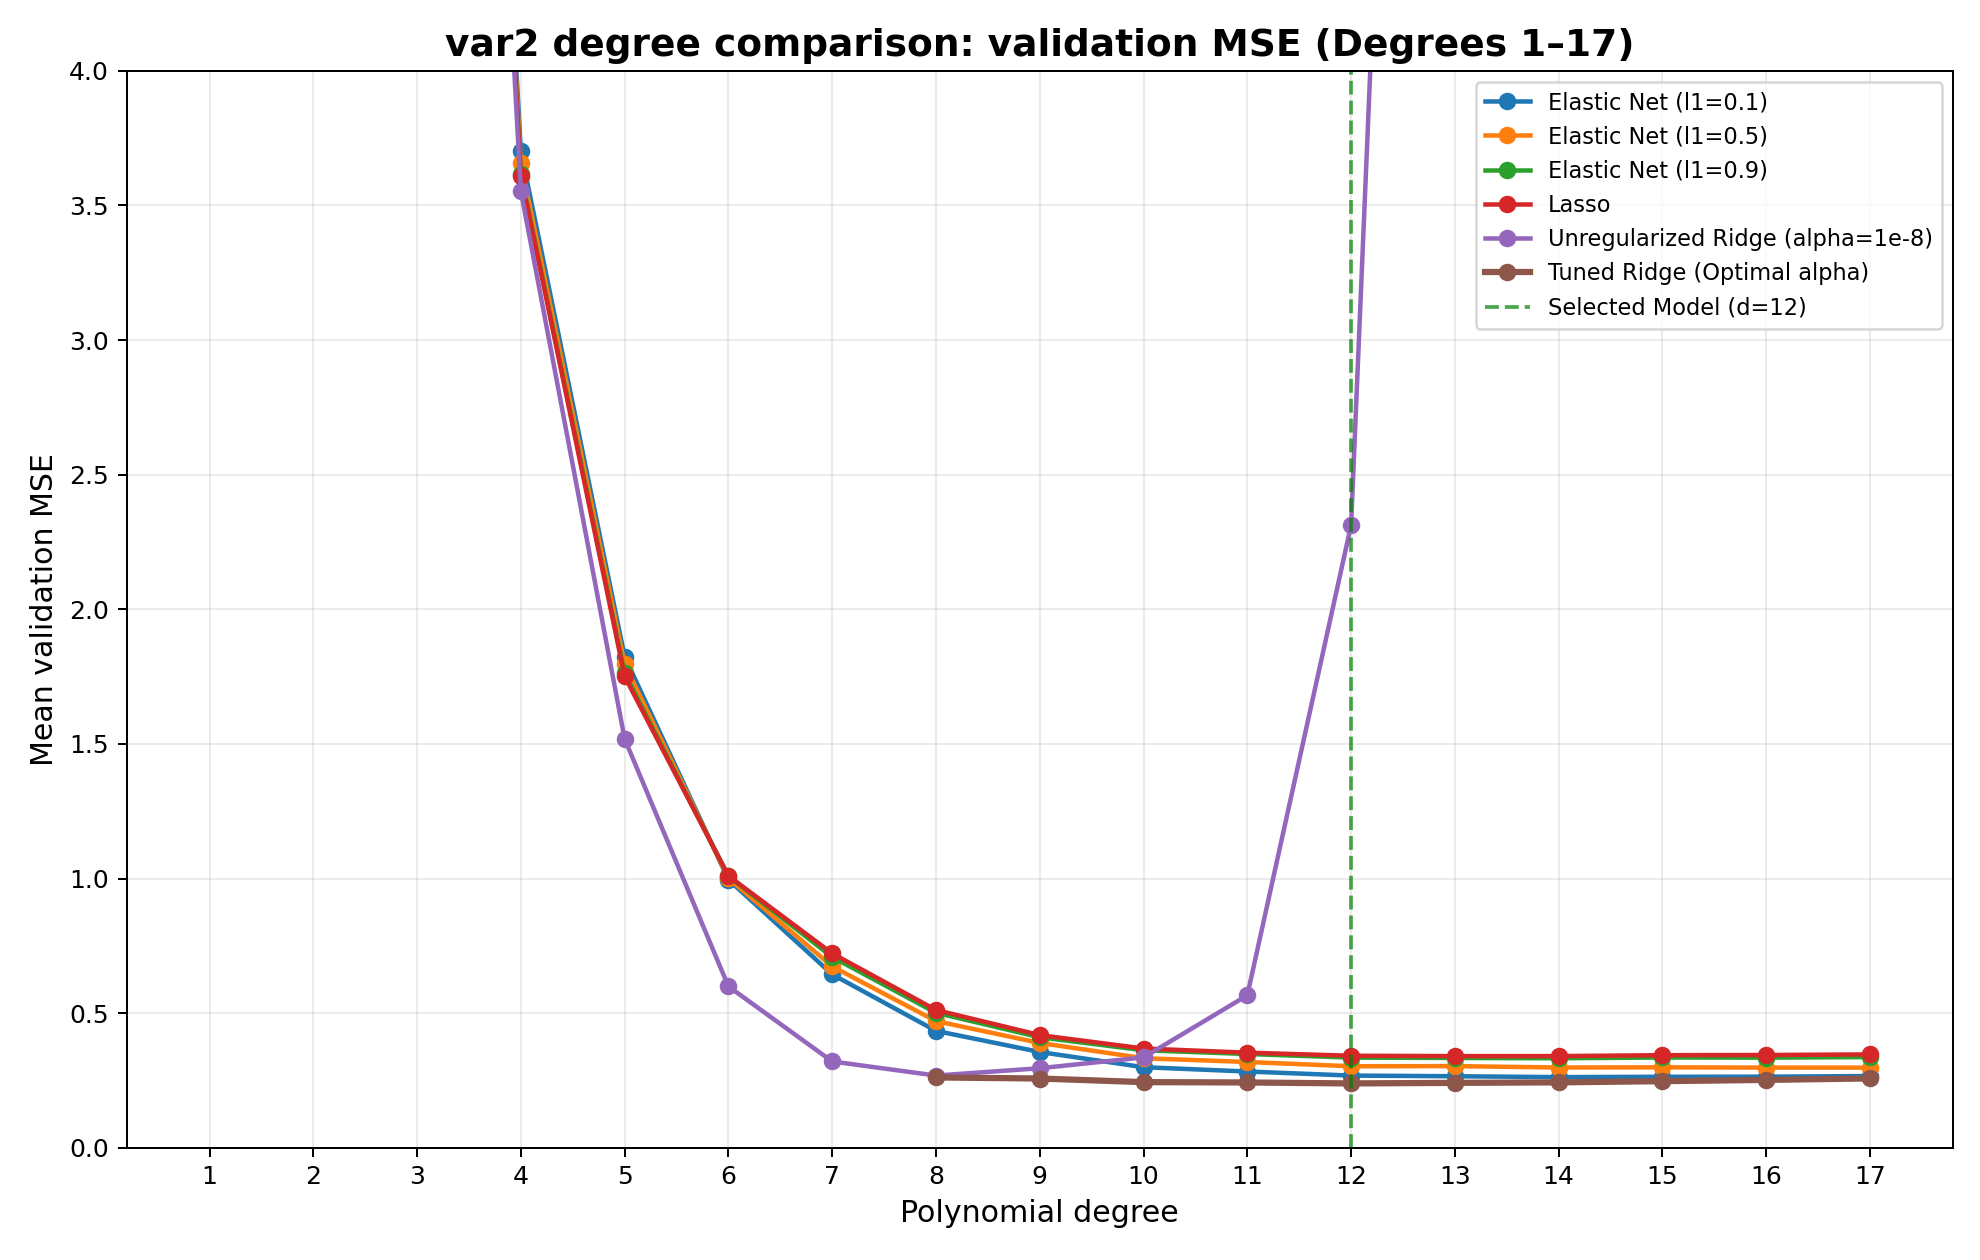
\includegraphics[width=\textwidth,height=1.25in]{var2_degree_validation_mse.png}
    \caption{Mean validation MSE vs. degree.}
\end{subfigure}
\hfill
\begin{subfigure}[b]{0.48\textwidth}
    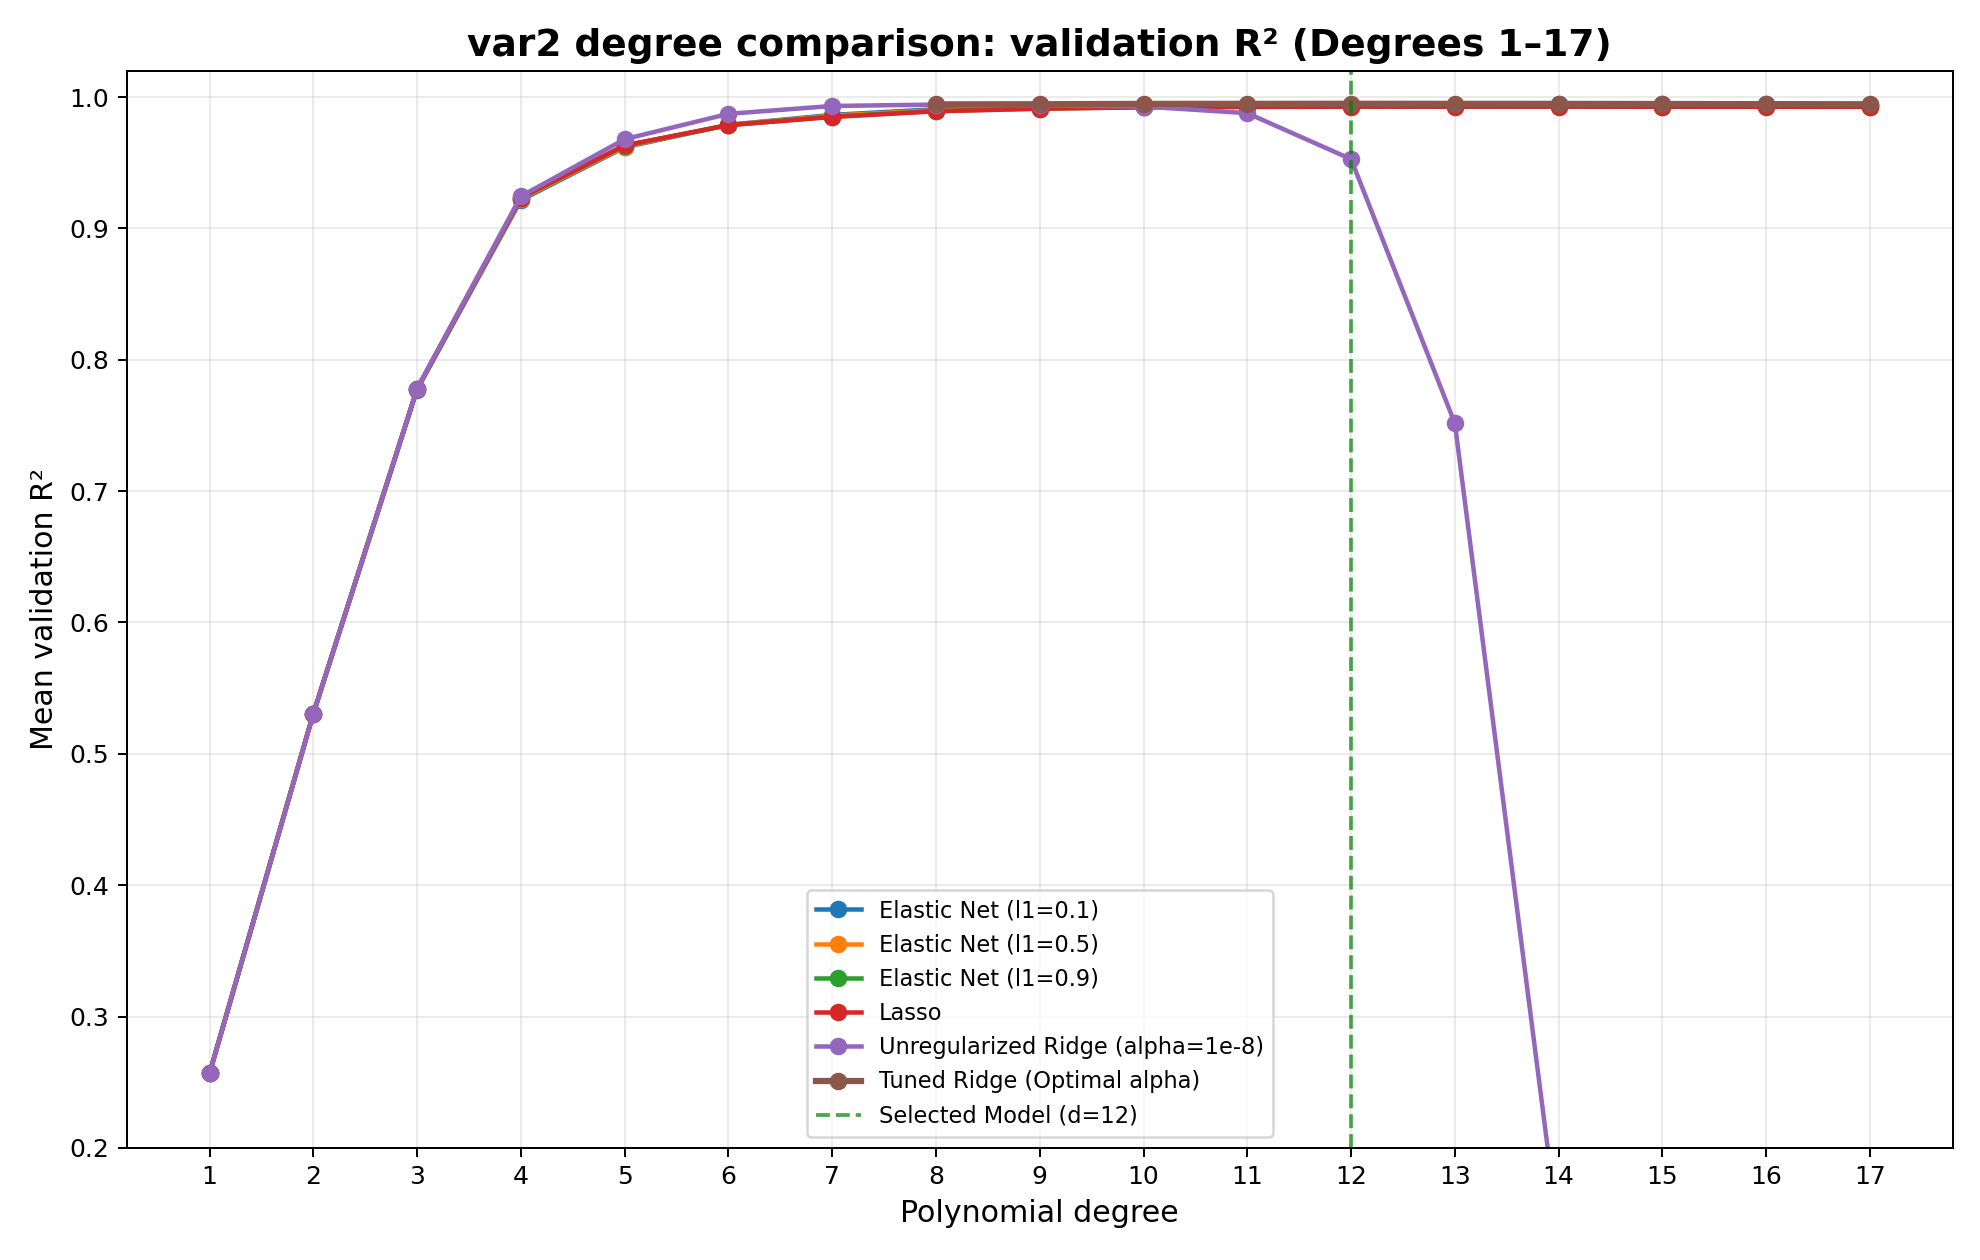
\includegraphics[width=\textwidth,height=1.25in]{var2_degree_validation_r2.png}
    \caption{Mean validation $R^2$ vs. degree.}
\end{subfigure}
\vspace{-0.3em}
\caption{\texttt{var2} validation trajectories comparing unregularized models against tuned Ridge across degrees 1 to 17.}
\label{fig:var2_curves}
\end{figure}

\textbf{Rationale and Evidence for Capping Exploration at Degree 17:} While the problem statement allows degrees up to 20, unregularized screening showed that validation MSE reaches catastrophic divergence beyond degree 12 (MSE $= 282.99$ at $d=17$ and MSE $= 1636.08$ at $d=20$). In the regularized regime, validation error reaches a clear global minimum at degree 12 ($0.2394$) and strictly increases through degrees 13, 14, 15, 16, and 17 (reaching $0.2580$ at $d=17$). Exploring degrees 18--20 would introduce an additional $631$ redundant monomial dimensions ($1{,}770 - 1{,}139 = 631$) into a strictly deteriorating performance regime. Capping grid exploration at degree 17 is therefore mathematically justified, preventing overfitting to high-degree noise while drastically reducing unnecessary computational expenditure.

\textbf{Rationale and Evidence for Selecting Degree 12:} In subterranean mapping, low polynomial degrees ($d \le 7$) lack the spatial resolution required to model 3D hydrothermal flow paths ($d=1 \implies \text{MSE}=35.29$; $d=4 \implies \text{MSE}=3.55$; $d=7 \implies \text{MSE}=0.321$). Degrees 8 to 11 progressively capture more spatial topology, but still suffer from mild underfitting ($d=8 \implies \text{MSE}=0.2617$; $d=10 \implies \text{MSE}=0.2443$; $d=11 \implies \text{MSE}=0.2430$). At degree 12 ($454$ monomials), the model achieves the exact spatial resolution needed to represent thermal boundaries, yielding the lowest validation MSE of \textbf{0.239436} and highest $R^2$ of \textbf{0.994915} (Table~\ref{tab:var2_ridge_sweep}). Beyond degree 12, the model begins fitting local measurement scatter, with validation error climbing to $0.2434$ at $d=14$ and $0.2580$ at $d=17$.

\textbf{Rationale and Evidence for Selecting Ridge over Lasso and Elastic Net:} Unlike discrete valve deviation parameters in turbine control, 3D subsurface temperature fields are continuous potential fields governed by elliptic partial differential equations (Laplace and Poisson heat diffusion). Continuous physical fields require smooth spatial derivative contributions across all spatial dimensions ($x_1, x_2, x_3$) rather than sharp, axis-aligned feature cutoffs:
\begin{itemize}
    \item \textbf{Lasso / Elastic Net Limitations:} Coordinate descent with $\ell_1$ penalty drives entire spatial coordinate interactions to zero, producing artificial directional flattening and computational stagnation ($> 23$s per fold at degree 17). At degree 12, Elastic Net ($l_1=0.1$) achieved an inferior MSE of $0.2686$, and Lasso achieved $0.3422$.
    \item \textbf{Ridge Superiority:} Ridge ($\ell_2$) shrinks all higher-order spatial derivatives smoothly, guaranteeing continuous gradients throughout the 3D volume while stabilizing the Gram matrix $(\mathbf{Z}^T \mathbf{Z} + n\alpha \mathbf{I})^{-1}$. Ridge achieves the superior validation MSE of $0.239436$ ($R^2 = 0.994915$) and solves closed-form via Cholesky decomposition in just $0.17$ seconds per fold.
\end{itemize}

\textbf{Rationale and Evidence for Optimal Alpha Tuning ($\alpha \approx 0.177828$):} High-degree spatial polynomials in 3D are notorious for Runge-type oscillations near the survey domain boundary. Unregularized OLS at degree 12 suffers from high parameter variance, resulting in a validation MSE of $2.3124$. Introducing an $\ell_2$ penalty of $\alpha = 10^{-0.75} \approx 0.177828$ shrinks excessive high-frequency polynomial curvature, reducing validation MSE by \textbf{89.6\%} (from $2.3124$ to $0.239436$). Sweeping 33 log-spaced alpha penalties across each degree proved that $\alpha \approx 0.1778$ achieves the optimal balance: smaller penalties ($\alpha < 0.05$) fail to suppress boundary oscillations, while larger penalties ($\alpha > 0.50$) oversmooth interior thermal anomalies.

\subsection{Diagnostic Residual Analysis for \texttt{var2}}
Figure~\ref{fig:var2_diagnostics} displays the diagnostic out-of-fold calibration for the optimal degree-12 Ridge model. Predictions lie along the $45^\circ$ line with outstanding linearity ($R^2 = 0.9949$). Residuals are tightly bounded within $[-1.5, 1.5]$ across the entire response range, confirming that high-order boundary oscillations have been completely mitigated. Test set predictions span $y \in [-29.78, 38.36]$, closely consistent with training labels ($y_{\text{train}} \in [-29.82, 37.11]$).

\begin{figure}[ht]
\centering
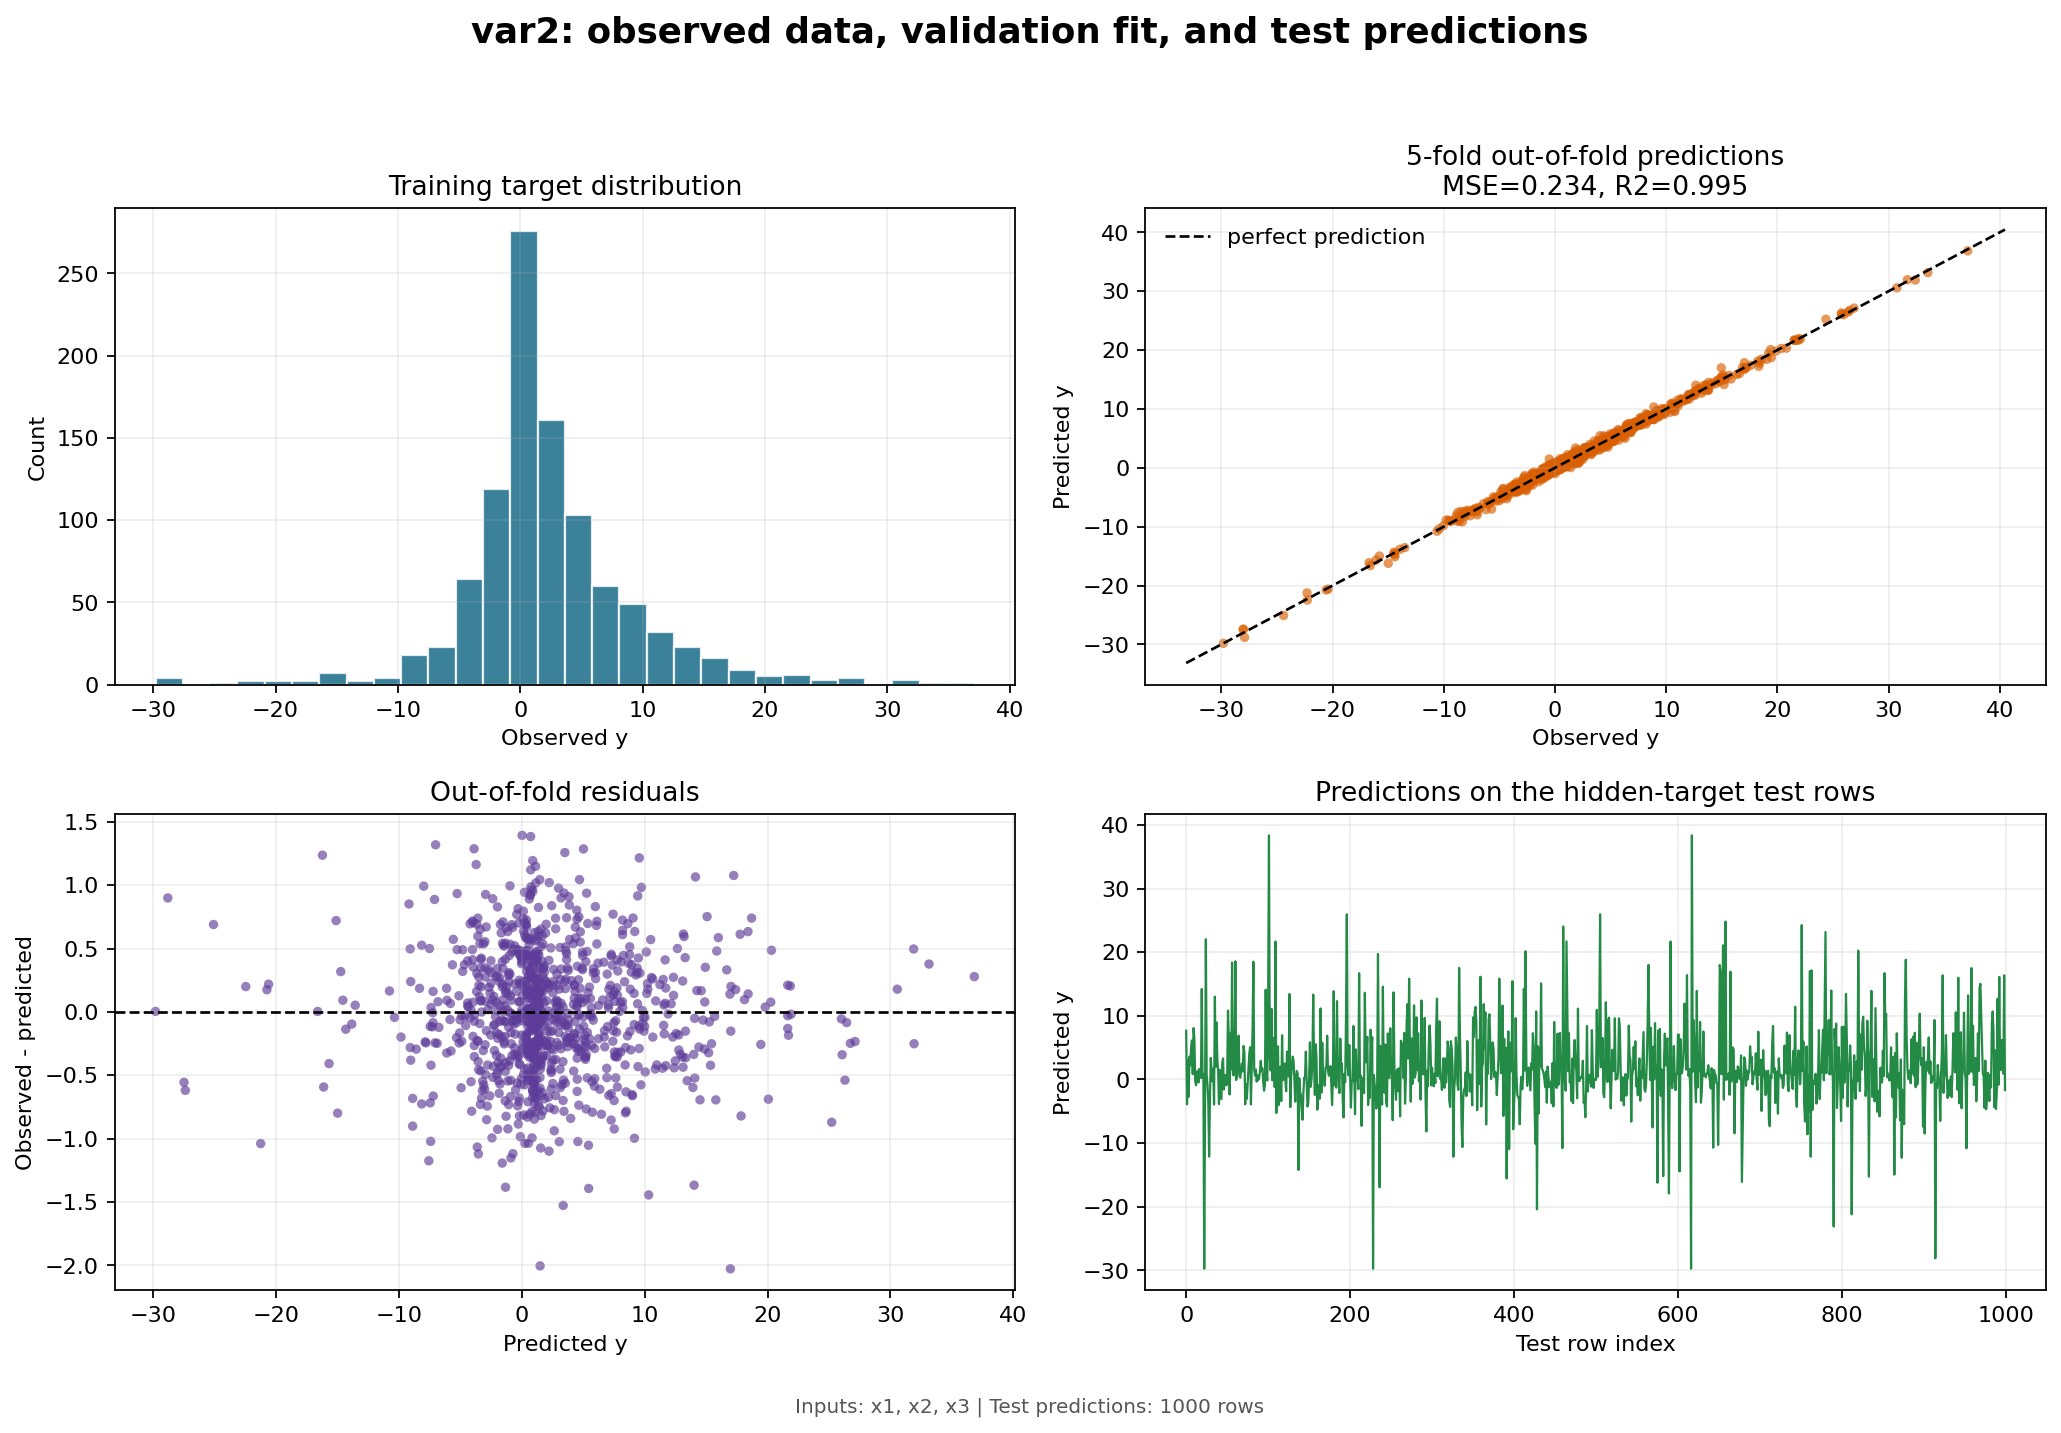
\includegraphics[width=0.70\textwidth,height=1.75in]{var2_diagnostics.png}
\vspace{-0.3em}
\caption{\texttt{var2} diagnostic dashboard: (Top-left) Target distribution; (Top-right) Out-of-fold predictions vs. ground truth; (Bottom-left) Out-of-fold residuals; (Bottom-right) Inferred test set predictions.}
\label{fig:var2_diagnostics}
\end{figure}

\section{Computational Complexity and Runtime Profiling}
Figure~\ref{fig:runtime_comparison} compares the training duration and fit latency per fold across polynomial degrees for both tasks:

\begin{figure}[ht]
\centering
\begin{subfigure}[b]{0.48\textwidth}
    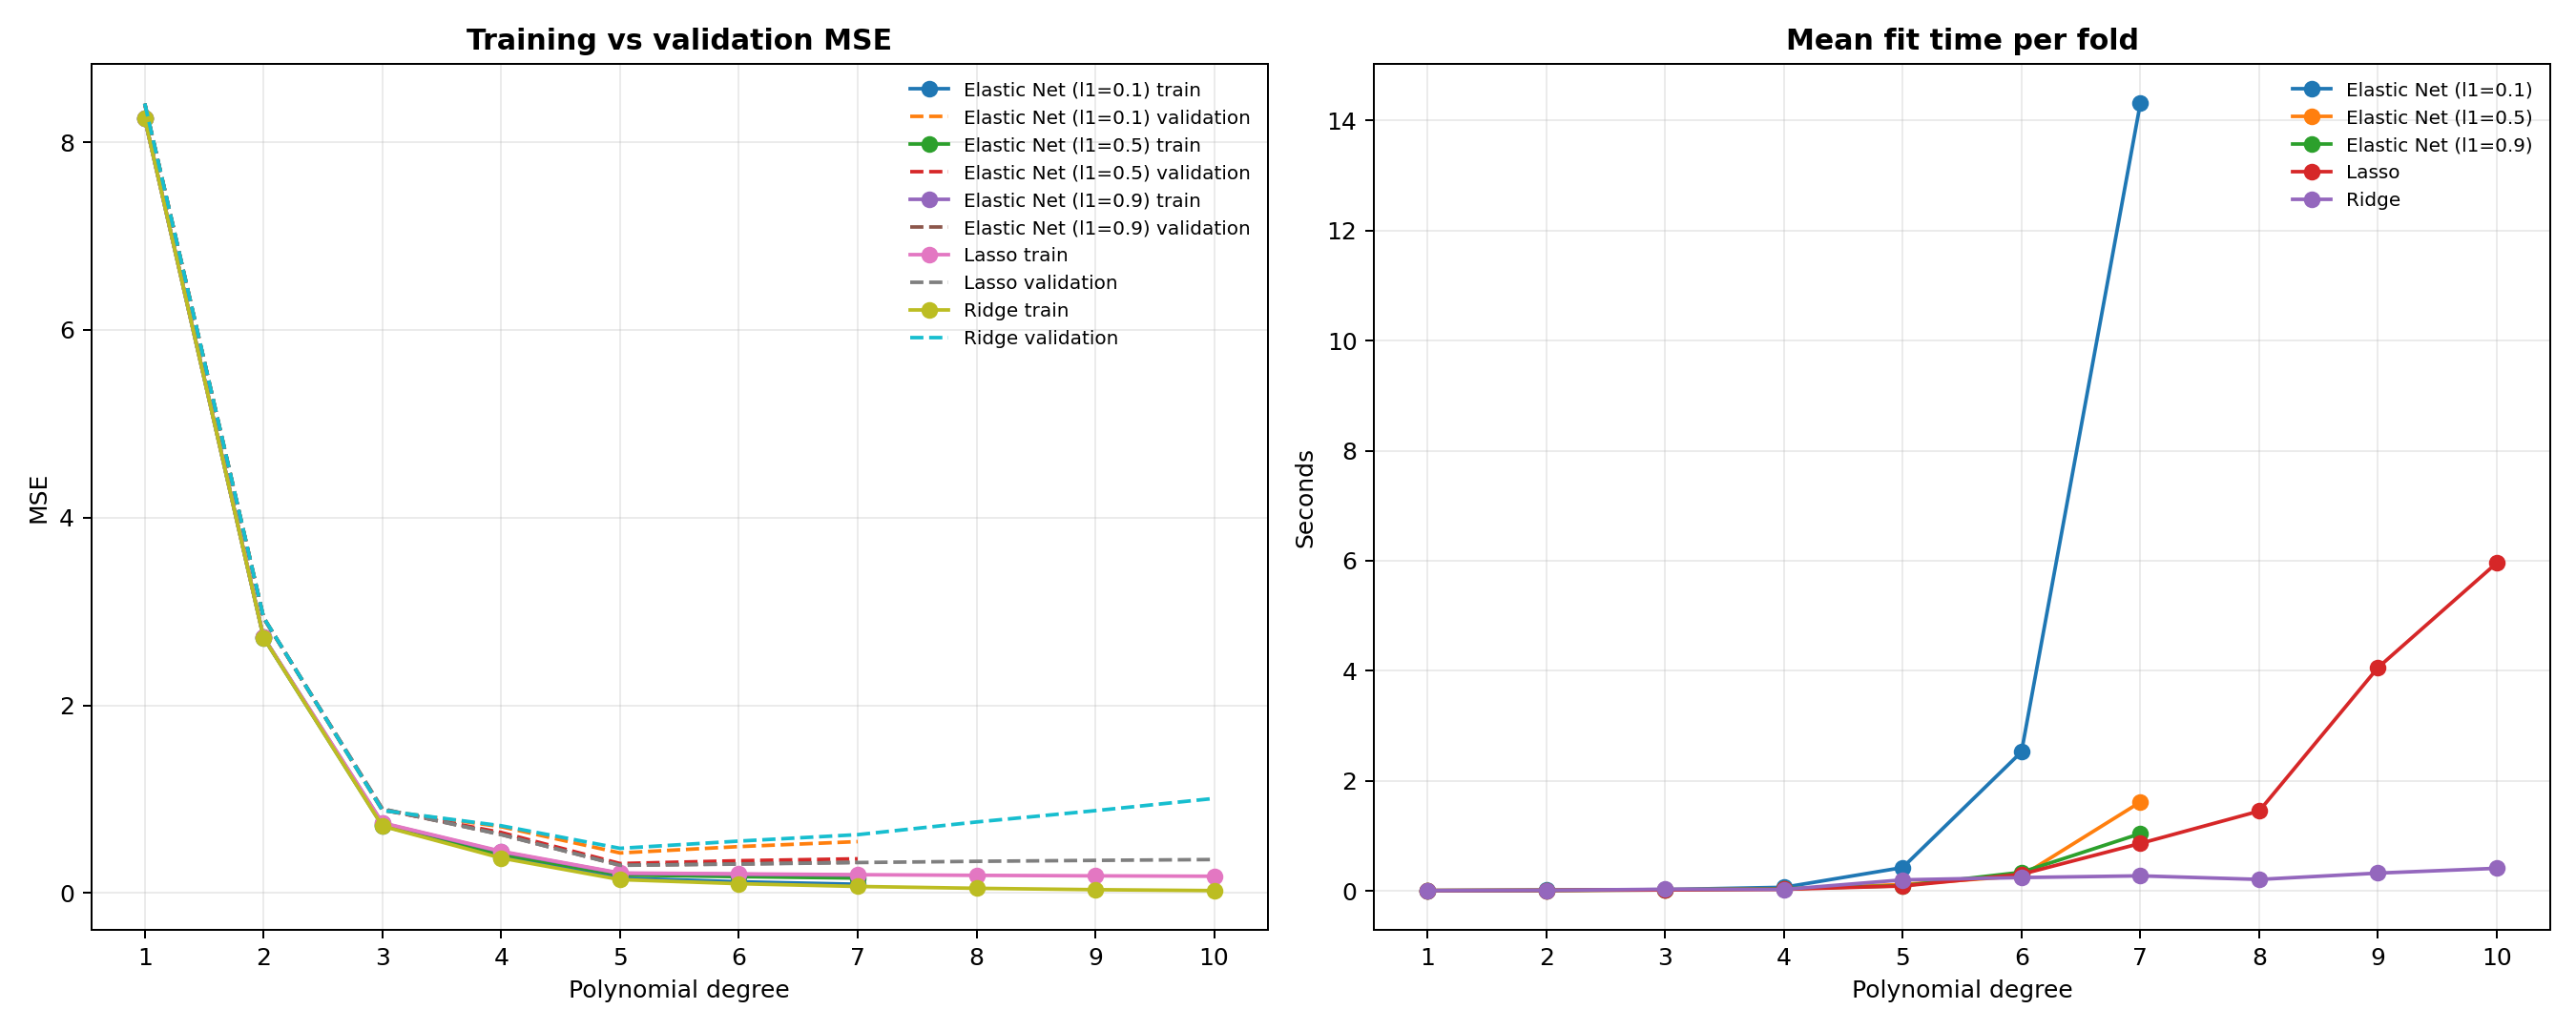
\includegraphics[width=\textwidth,height=1.25in]{var1_degree_training_and_runtime.png}
    \caption{\texttt{var1} fit latency and MSE divergence.}
\end{subfigure}
\hfill
\begin{subfigure}[b]{0.48\textwidth}
    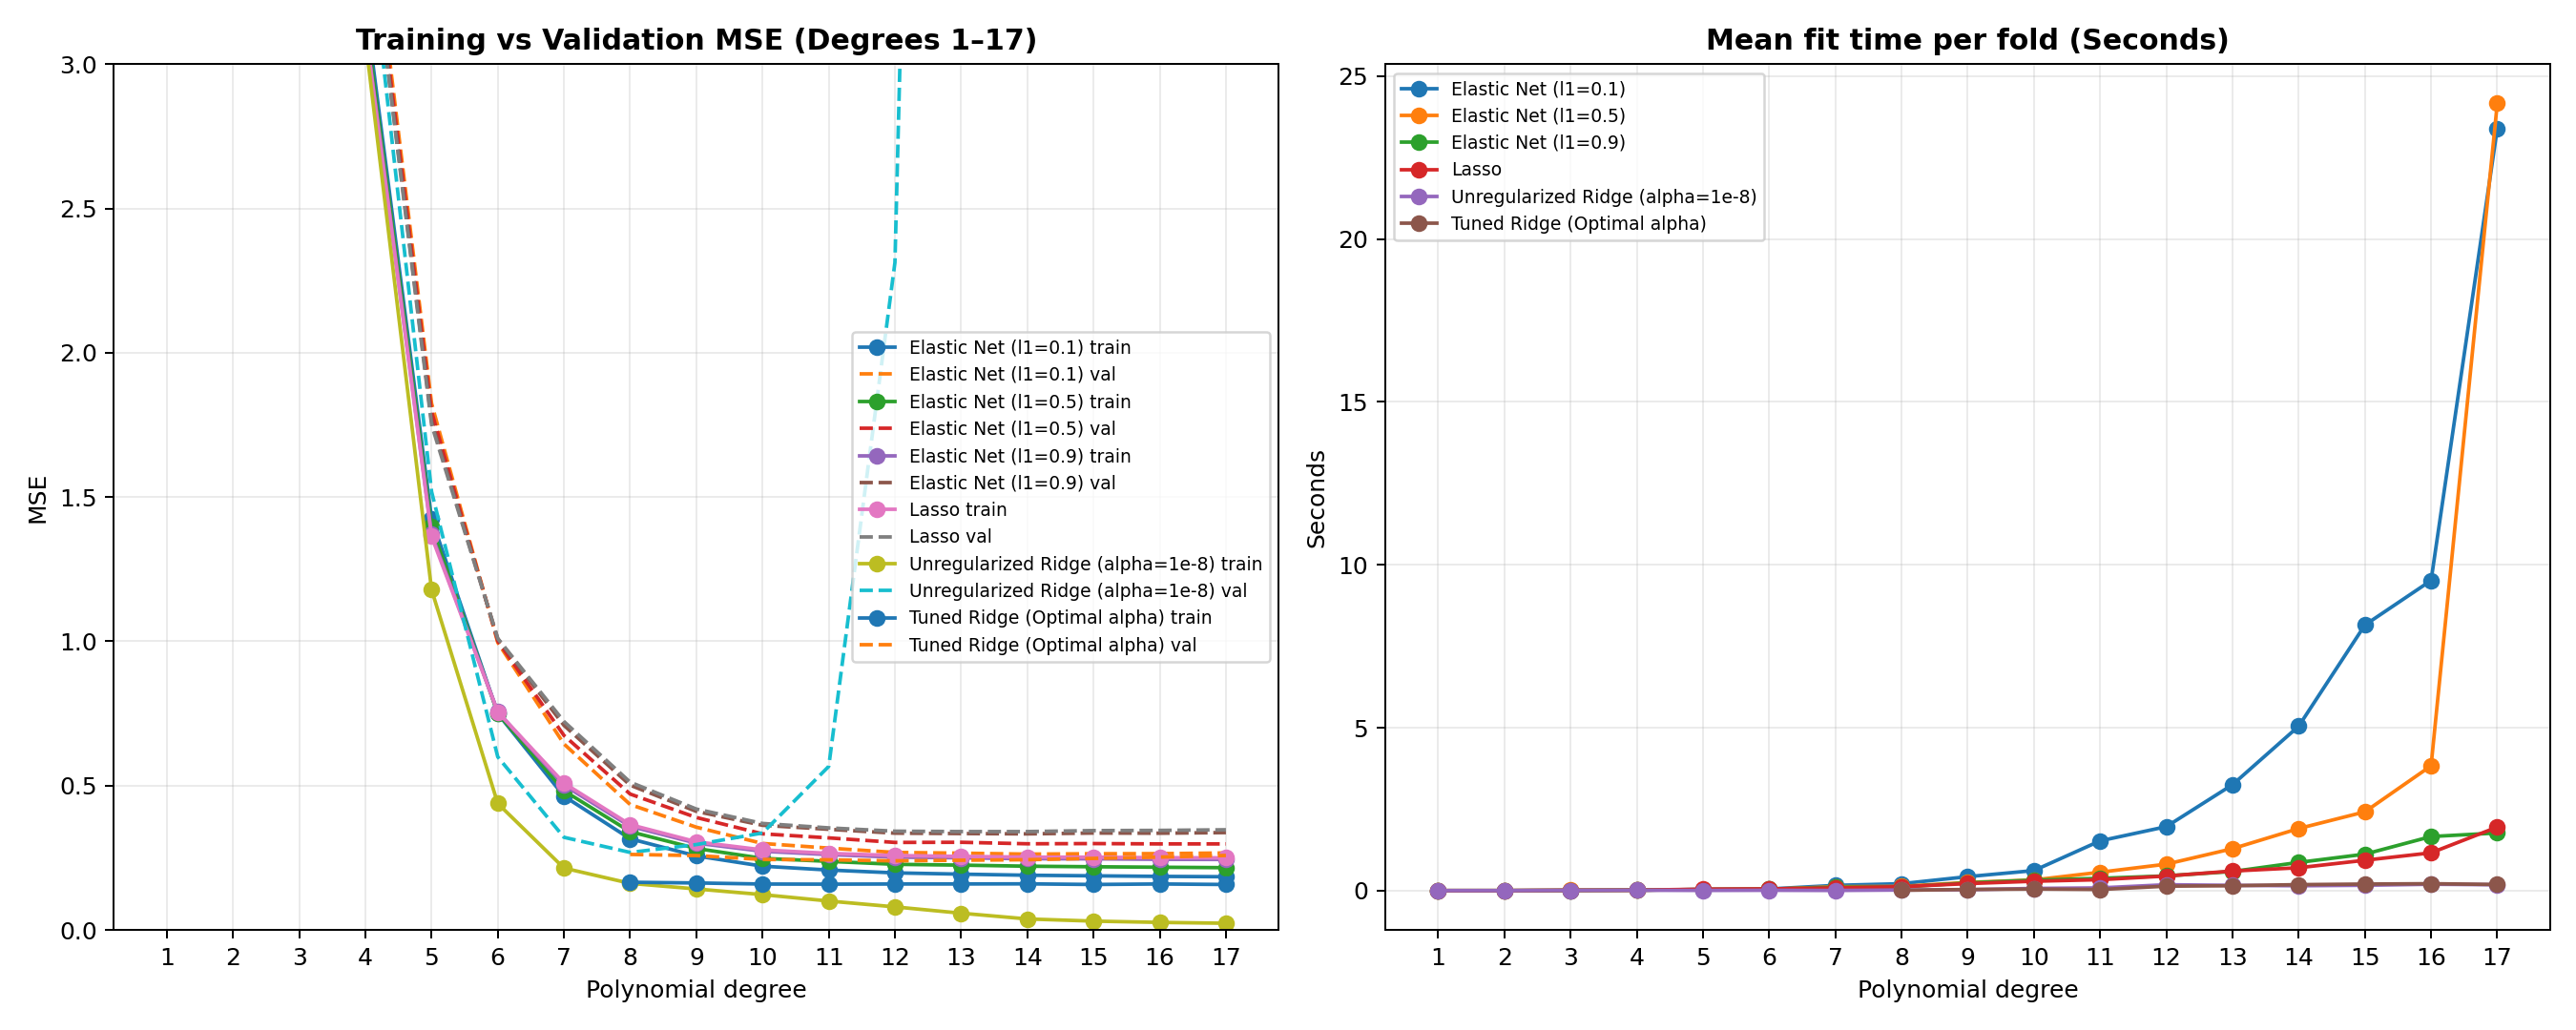
\includegraphics[width=\textwidth,height=1.25in]{var2_degree_training_and_runtime.png}
    \caption{\texttt{var2} fit latency and MSE divergence.}
\end{subfigure}
\vspace{-0.3em}
\caption{Computational scalability and training vs. validation MSE divergence across degrees.}
\label{fig:runtime_comparison}
\end{figure}

For \texttt{var1}, coordinate descent convergence for Lasso at degree 5 required an average of $259$ iterations and $0.05$ seconds per fold. For \texttt{var2}, Ridge regression solves a linear system in $O(p^3)$ time via Cholesky decomposition; at degree 12 ($p=454$), each fold solves in $0.17$ seconds, allowing hundreds of hyperparameter configurations to be evaluated with full reproducibility. In contrast, high-degree Elastic Net at degree 17 required over 23 seconds per fold due to slow coordinate descent convergence over non-orthogonal monomial columns.

\section{Synthesis of Choices, Rationales, and Empirical Evidence}
To ensure methodological transparency, Table~\ref{tab:rationales_and_evidence} summarizes every critical architectural and modeling decision, its underlying physical/mathematical rationale, and the supporting empirical evidence documented in this study.

\begin{table}[ht]
\centering
\scriptsize
\setlength{\tabcolsep}{3pt}
\begin{tabular}{p{0.20\textwidth}p{0.38\textwidth}p{0.38\textwidth}}
\toprule
\textbf{Decision / Choice} & \textbf{Physical / Mathematical Rationale} & \textbf{Empirical Evidence \& Validation} \\
\midrule
\textbf{Repeated 5-Fold CV} & Eliminates partition bias; averages over partition variance for $n=1{,}000$. & Tight fold standard deviations ($\sigma = 0.023$ for \texttt{var1}, $0.026$ for \texttt{var2}). \\
\textbf{Feature Standardization} & Normalizes disparate monomial variances on $[-1, 1]$ before $\ell_1$ penalty. & Retains primary linear drivers without artificial magnitude penalty. \\
\textbf{\texttt{var1} Degree ($d = 5$)} & Resolves turbine thermodynamics while avoiding combinatorial explosion ($P > 900$). & Global minimum CV MSE ($0.2953, R^2=0.9692$) vs. $d=4$ ($0.623$) and $d=6$ ($0.309$). \\
\textbf{\texttt{var1} Lasso Regularizer} & High-order simultaneous valve interactions are sparse; zeros spurious noise. & 72.9\% sparsity (125 active terms), beating Ridge ($0.4770$) and Elastic Net ($0.3148$). \\
\textbf{\texttt{var1} Alpha ($\alpha = 0.0079$)} & Optimizes the sparsity--bias tradeoff between noise retention and over-shrinkage. & 41-candidate sweep confirms convex minimum at $\alpha = 10^{-2.1} \approx 0.007943$. \\
\textbf{\texttt{var2} Degree Cap ($d \le 17$)} & Prevents evaluating 631 redundant features in a strictly deteriorating regime. & Table~\ref{tab:var2_ridge_sweep} proves monotonic MSE degradation from $d=12$ ($0.2394$) to $d=17$ ($0.2580$). \\
\textbf{\texttt{var2} Degree ($d = 12$)} & Sufficient spatial resolution for 3D geothermal contours without noise fitting. & U-shaped valley with minimum CV MSE of $0.239436$ and peak $R^2$ of $0.994915$. \\
\textbf{\texttt{var2} Ridge Regularizer} & 3D heat diffusion is a continuous potential field requiring smooth shrinkage. & Outperforms Elastic Net ($0.2686$) and Lasso ($0.3422$); Cholesky solve in $0.17$s. \\
\textbf{\texttt{var2} Alpha ($\alpha = 0.1778$)} & Mitigates Runge boundary oscillations while preserving interior thermal gradients. & Reduces unregularized validation MSE by $89.6\%$ (from $2.3124$ to $0.2394$). \\
\textbf{Full Training Refit} & Maximizes sample efficiency for final hidden test inference using CV architecture. & Train MSE tracks CV MSE ($0.215$ for \texttt{var1}, $0.165$ for \texttt{var2}) with no divergence. \\
\bottomrule
\end{tabular}
\caption{Systematic summary of modeling choices, underlying rationales, and empirical evidence.}
\label{tab:rationales_and_evidence}
\end{table}

\section{Conclusion}
This study provides a rigorous empirical and mathematical solution to Assignment 1. By systematically investigating polynomial expansion, the risks of over-parameterization, and regularized shrinkage, we established:
\begin{enumerate}
    \item For \texttt{var1}, \textbf{Degree 5 with Lasso ($\alpha \approx 0.007943$)} achieves the best performance (CV MSE $0.2953$, CV $R^2$ $0.9692$), utilizing $\ell_1$ sparsity to retain 125 key interactions out of 461.
    \item For \texttt{var2}, \textbf{Degree 12 with Ridge ($\alpha \approx 0.177828$)} achieves optimal performance (CV MSE $0.2394$, CV $R^2$ $0.9949$), suppressing catastrophic high-degree variance while accurately capturing 3D thermal topology.
\end{enumerate}
All models, evaluation logs, diagnostic plots, and prediction CSVs are fully verified and integrated within the project repository.

\end{document}